\documentclass[12pt]{amsart}
\usepackage{latexsym}
\usepackage{amssymb,amsmath}
\usepackage[pdftex]{graphicx}
\usepackage{enumerate}
\usepackage{endnotes}
%\usepackage{extpfeil}
\usepackage{hyperref}
\usepackage[usenames,dvipsnames]{xcolor}
\usepackage{stackrel}
\usepackage{bbm}
\usepackage{tikz}
\usepackage[margin=1.25in]{geometry}
\usepackage{hyperref}
\usepackage{listings}
\usepackage{courier}
\usepackage{color}

\lstset{
	basicstyle=\small\ttfamily,
	keywordstyle=\color{blue},
	language=python,
	xleftmargin=16pt,
}

\usetikzlibrary{arrows,chains,matrix,positioning,scopes}

\makeatletter
\tikzset{join/.code=\tikzset{after node path={%
\ifx\tikzchainprevious\pgfutil@empty\else(\tikzchainprevious)%
edge[every join]#1(\tikzchaincurrent)\fi}}}
\makeatother
%
\tikzset{>=stealth',every on chain/.append style={join},
         every join/.style={->}}
\tikzstyle{labeled}=[execute at begin node=$\scriptstyle,
   execute at end node=$]
\usetikzlibrary{patterns}

\usetikzlibrary{decorations.pathreplacing}

\DeclareSymbolFont{bbold}{U}{bbold}{m}{n}
\DeclareSymbolFontAlphabet{\mathbbold}{bbold}

\newtheorem{thm}{Theorem}[section]
\newtheorem{ithm}{Theorem}
\newtheorem{lem}[thm]{Lemma}
\newtheorem{prop}[thm]{Proposition}
\newtheorem{cor}[thm]{Corollary}

\theoremstyle{definition}
\newtheorem{defi}[thm]{Definition}
\newtheorem{example}[thm]{Example}
\newtheorem{exercise}[thm]{Exercise}
\newtheorem{rem}[thm]{Remark}


   
\def\B{{\mathbb B}}
\def\C{{\mathbb C}}
\def\D{{\mathbb D}}
\def\Fp{{\mathbb F}_p}
\def\Fell{{\mathbb F}_{\ell}}
\def\F{{\mathbb F}}
\def\H{{\mathbb H}}
\def\M{{\mathbb M}}
\def\N{{\mathbb N}}
\def\O{{\mathcal O}}
\def\0{{\mathbb 0}}
\def\P{{{\mathbb P}}}
\def\Q{{\mathbb Q}}
\def\R{{\mathbb R}}
\def\T{{\mathbb T}}
\def\Z{{\mathbb Z}}

\newcommand{\sol}{_{a^p,b^p,c^p}}
\newcommand{\bound}{\partial}
\newcommand{\la}[1]{\mathfrak{#1}}
\newcommand{\im}{\text{Im} \hspace{0.1em} }
\newcommand{\ann}{\text{Ann} \hspace{0.1em} }
\newcommand{\rank}{\text{rank} \hspace{0.1em} }
\newcommand{\coker}[1]{\text{coker}\hspace{0.1em}{#1}}
\newcommand{\sgn}{\text{sgn}}
\newcommand{\lcm}{\text{lcm}}
\newcommand{\re}{\text{Re}  \hspace{0.1em} }
\newcommand{\ext}[1]{\text{Ext}(#1)}
\newcommand{\Hom}[1]{\text{Hom}(#1)}
\newcommand{\End}[1]{\text{End(#1)}}
\newcommand{\bs}{\setminus}
\newcommand{\rpp}[1]{\mathbb{R}\text{P}^{#1}}
\newcommand{\cpp}[1]{\mathbb{C}\text{P}^{#1}}
\newcommand{\tr}{\text{tr}\hspace{0.1em} }
\newcommand{\inner}[1]{\langle {#1}\rangle}
\newcommand{\tensor}{\otimes}
\newcommand{\Cl}{\text{Cl}}
\renewcommand{\sp}[1]{\text{Sp}_{#1}}
\newcommand{\GL}{\text{GL}}
\newcommand{\pgl}[1]{\text{PGL}_{#1}}
\renewcommand{\sl}[1]{\text{SL}_{#1}}
\newcommand{\so}[1]{\text{SO}_{#1}}
\newcommand{\SO}{\text{SO}}
\newcommand{\pso}[1]{\text{PSO}_{#1}}
\renewcommand{\o}[1]{\text{O}_{#1}}
\renewcommand{\sp}[1]{\text{Sp}_{#1}}
\newcommand{\psp}[1]{\text{PSp}_{#1}}
\newcommand{\Span}{\rm Span}
\newcommand{\Frob}{\rm Frob}
\newcommand{\tor}{\rm tor}
\newcommand{\rad}{\rm rad}
\newcommand{\denom}{\rm denom}
\renewcommand{\bar}{\overline}
\newcommand{\notdiv}{\nmid}
\newcommand{\pfrac}[2]{\left( \frac{#1}{#2} \right)}
\newcommand{\Ell}{\rm Ell}
\newcommand{\AV}{\rm AV}

\newcommand{\kron}[2]{\bigl(\frac{#1}{#2}\bigr)}
\newcommand{\leg}[2]{\Biggl(\frac{#1}{#2}\Biggr)}

\DeclareSymbolFont{bbold}{U}{bbold}{m}{n}
\DeclareSymbolFontAlphabet{\mathbbold}{bbold}

\begin{document}

\title{Perfect Powers in Lucas Sequences}
\author{Jesse Silliman and Isabel Vogt}

\maketitle

\section{Preliminaries}


We define a binary recurrence relation by the identifiers $(b,c)$ defining the relation
\[ u_{n+2} = b\cdot u_{n+1}+ c\cdot u_n. \]
To this we associate the characteristic polynomial
\[ g(z) = z^2 - bz - c\]
with roots
\[ \alpha, \beta = \frac{b \pm \sqrt{b^2+4c}}{2}. \]
Specific binary recurrence sequences require the additional identifier of initial conditions $u_0$ and $u_1$.  We will be primarily interested in two companion sequences for a given recurrence relation $(b,c)$, which we will refer to as $u_n$ and $v_n$, specified by the starting conditions
\[ u_0 = 0, u_1 = 1 \qquad \qquad v_0 = 2, v_1 = b \]
The $n$th terms of these sequence are specified by the formulas
\[u_n = \frac{\alpha^n - \beta^n}{\alpha - \beta} \qquad \qquad v_n = \alpha^n +\beta^n \]
It is straightforward to verify the following facts
\begin{equation}\label{fib2} u_{2k} = u_kv_k \end{equation}
\begin{equation}\label{gen_diophan}(\alpha - \beta)^2u_n^2 = v_n^2 - 4(\alpha\beta)^n \end{equation}
The second fact in the list allows us to generate Frey curves.  In particular, say that we posit a solution $u_n = y^p$, that is
\begin{equation}\label{rel_diophan} (b^2+4c)y^{2p}+4(-c)^n = v_n^2 .\end{equation}
This is a solution to the diophantine equation
\[ (b^2+4c)X^p +4(-c)^nY^p = Z^2 \]
$(p,p,2)$ with nontrivial coefficients.

\section{Results for Specific Sequences}

\begin{thm}[No Newforms]\label{noforms1}
Let $u_n$ be the binary recursion sequence defined by 
\[ u_{n+2} = bu_{n+1} +cu_n \]
with $b^2+4c = 1$ and initial conditions $u_0 = 0$ and $u_1=1$.  Then for the following values of $b$ and $c$:
\begin{center}
\begin{tabular}{c | c }
b & c \\  \hline \hline
3 & -2 \\
5 & -6  \\
7 & -12 \\
17 & -72  \\
9 & -20 \\ \hline \hline
\end{tabular}
\end{center}
$u_n$ has no nontrivial $p$th powers, except perhaps for 5th powers in $(9,-20)$.
\end{thm}

In order to prove the above theorem we first establish the following lemmas.

\begin{lem}\label{relprime}
Let $b^2+4c=1$.  For $n \geq 1$,  $u_n$, $v_n$, and $c$ are relatively prime.
\end{lem}

\begin{proof}
We prove this by induction.  First note that $b^2 +4c = 1$ forces $b$ and $c$ to be relatively prime and $c$ to be even.  Clearly as
\[ u_2 = b \cdot u_1 + c \cdot u_0 \]
and $u_1$ is relatively prime to $c$, $u_2$ is relatively prime to $c$.  Thus by induction $u_n$ is relatively prime to $c$.  Similarly for $v_n$.  And further as $u_n^2  = v_n^2 - 4(-c)^n$, no primes except perhaps those dividing $c$ can divide $u_n$ and $v_n$.  Thus they are pairwise relatively prime.
\end{proof}

\begin{lem}[Ruling out small primes]\label{smallp}
There are no nontrivial squares or cube terms in any of the above examples except $u_2 = 9$ for the sequence $(9,-20)$.
\end{lem}

\begin{proof}

We first deal with the case of $p=2$; we will derive our contradiction from the relation \eqref{gen_diophan}, which in this case reduces to
\begin{equation}\label{D1dio} \alpha^n - (\alpha-1)^n = z^2.\end{equation} 
Assume that the index $n$, for which $u_n = z^2$, is odd; in this case we can absorb the sign and have a nontrivial solution to
\begin{equation}\label{diophanpp2}
x^n +y^n = z^2
\end{equation}
But there are no nontrivial solutions to \eqref{diophanpp2} (cite merel + darmon) for $n \geq 4$.  We easily check that there are no solutions for $n=3$.  In the case $n$ is even, write $n=2^rk$ for $k$ odd.  Then we can write
\[ \alpha^{2^rk} - \beta^{2^rk} = (\alpha^{2^{r-1}k} - \beta^{2^{r-1}k}) (\alpha^{2^{r-1}k} + \beta^{2^{r-1}k}) \cdots (\alpha^{k} - \beta^{k}) (\alpha^{k} + \beta^{k}). \]
Further by lemma \ref{relprime}, we know that that these terms are relatively prime.  Thus $u_n=z^2$ if and only if each of these terms is also a square.  In particular, $\alpha^k + \beta^k$ must be a square.  If $k \neq 1$, then this is identical to the previous condition, which yields a contradiction.  If $k = 1$, then this is the condition that $b$ is a perfect square.  It is easy to verify that this is not true in all of the above examples, except $(9,-20)$.  The proof for $p=3$ follows in exactly the same way from reduction to odd index and the solution of $(n,n,3)$ by (cite Darmon and Merel).

\end{proof}


\begin{proof}[Proof of Theorem \ref{noforms1}]
Posit a solution $u_n = y^p$ for $n \geq 5$ and $p \geq 7$.  We have a Diophantine equation
\[ y^{2p} + 4(-c)^n = v_n^2. \] 
By lemma \ref{relprime} the solution $(y^2, 1, v_n)$ is a primitive solution to 
\[ X^p + 4(-c)^n Y^p = Z^p.\]
To this hypothetical solution we associate a Frey curve
\[E: Y^2 + XY = X^3 + \frac{w_n - 1}{4} X^2 + 2^{-4}c^nX \]
for $w_n = \pm v_n$ such that $w_n \equiv 1 \pmod{4}$; note that $2|c$.  This has conductor and minimal discriminant
\begin{equation}\label{conddis1} N_E =\prod_{\ell | cy} \ell  \qquad \qquad \Delta_E = 2^{-8} \cdot (-c)^{2n} \cdot y^{2p} \end{equation}
and the mod $p$ Galois representation $\rho_{E,p}$ is unramified outside $p\rad{(c)}$, by a Tate curve argument.  Further, as $p \notdiv c$, all of the ramification at $p$ comes from $\Q(\zeta_p)$, and thus it is flat at $p$.  By a theorem of Mazur it is irreducible for $p \geq 7$ (argued explicitly in (cite Bennett and Skinner)).  By Ribet's level-lowering theorem, the representation $\rho_{E,p}$ is isomorphic to one arising from a modular form of level $N = \rad(c)$.  For $b,c$ as above, there are no modular forms of level $\rad(c)=2,6,10$.  So there are no perfect $p$th powers if $p \geq 7$.

Excluding the last example where $5|c$, the only obstruction to the validity of the above argument at the prime $5$ is that we cannot immediately conclude that $\rho_{E,5}$ is irreducible.  If $\rho_{E,5}$ were reducible, it would give rise to a rational point on $X_0(5) \simeq \P_1$.  Let $X_{\Delta} \simeq \P_1$ be the degree $2$ cover of $X(1)$ parameterizing an elliptic curve $E'$ and a choice of square root of its discriminant $\Delta_{E'}$.  The map to $X(1)$ is given by
\[z \mapsto z^2 + 12^3. \]
The discriminants of our Frey curves given in \eqref{conddis1} are all rational squares.  Thus the Frey curves above correspond to rational points on $X_{\Delta}$.
As in (cite DZB) we construct the following diagram
\begin{center}
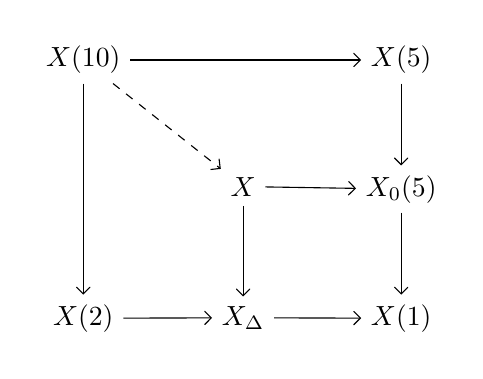
\begin{tikzpicture}[scale=2]
\matrix (m) [matrix of math nodes, row sep=3em, column sep=3em]
{ X(10) & & X(5)  \\
 & X & X_0(5)  \\
X(2) & X_{\Delta} & X(1)\\};
\path[->,font=\scriptsize,>=angle 90]
(m-1-1) edge  (m-3-1)
(m-1-1) edge (m-1-3)
(m-1-3) edge  (m-2-3)
(m-1-1) edge[dashed]  (m-2-2)
(m-2-3) edge  (m-3-3)
(m-2-2) edge  (m-2-3)
(m-2-2) edge  (m-3-2)
(m-3-1) edge  (m-3-2)
(m-3-2) edge  (m-3-3);
\end{tikzpicture}
\end{center}
where $X$ is the normalization of the fiber product $X_{\Delta} \times_{X(1)} X_0(5)$.  $X$ is an elliptic curve given by the equation
\[X: \qquad  y^2 = x^3 + 22x^2 +125x .\]
The map to $X_{\Delta}$ is given by
\[ (x,y) \mapsto \frac{y(x^2-500x -15625)}{x^3}. \]
Sage easily determines that $X$ is rank $0$, with rational point $(0:0:1)$ and $(0:1:0)$, both lying in the kernel of the map to $X_{\Delta}$.  Thus our Frey curve cannot give rise to a rational point on $X_0(5)$, and we conclude that $\rho_{E,5}$ is irreducible.  Thus a similar level lowering argument at $5$ works here to allow us to conclude that there are no nontrivial perfect $5$th powers.

Invoking lemma \ref{smallp} completes the proof of the theorem.
\end{proof}

\begin{rem}
The result for $b = 3, c = -2$ follows from Catalan's Conjecture on perfect powers that differ by one.
\end{rem}


\section{A general theorem}

For a binary recursion sequence $u_n$ characterized by $(b,c)$ relatively prime and starting conditions $u_0=0,u_1=1$, let $N = 2c * (b^2+4c)$.  Further let $\alpha,\beta$ be roots of the characteristic polynomial for $(b,c)$, with $\alpha$ the dominant root.  Define the bounds:
\begin{align*}
\Ell(N) & = \max\{30, N\}*\log{\alpha}/\log{2} \\
\AV(N) & \sim N^N. 
\end{align*}

\begin{lem}[Bound on Irrational Newforms]\label{irnewbound1}
Let $E$ be an elliptic curve of level $M \cdot N$ with mod-$p$ Galois representation $\rho_{E,p}$ irreducible, unramified outside $N$, and flat at $p$.
\end{lem}


\begin{thm}[Upper Bound on $p$]

\end{thm}
















\end{document}